\clearpage
\section{Targeted revisions and fresh held-out evaluations}
\label{sec:revisions}
\subsection{A new experiment, with the original failures retained}
Version 4 addresses the shared semantic errors and adaptive-memory harms observed in Section~\ref{sec:local-tests}. The entire version 3 manuscript, source archive, and computational evidence archive were copied to a separate preservation directory before editing. The original experiment files remain unchanged and are checked against a 257-file preservation manifest. The earlier results retain their original decisions and cannot be reclassified by improvements in a later algorithm. New code, development work, freezes, validation selections, held-out outcomes, and audits are separate artifacts \cite{revisiontests}.

This is an internally developed revision program. Earlier failures legitimately inform its design, so the twelve original semantic cases and earlier simulation paths are development evidence rather than fresh confirmation. The new semantic cases were authored by a separate AI agent that did not inspect the revised implementation; the implementation author did not inspect those cases before the freeze. This division reduces direct case leakage but does not provide independent human adjudication or independent underlying models. All new label judgments remain provisional. Memory tuning uses a separate validation bank, followed by a frozen selected configuration and disjoint test banks.

\subsection{Semantic revision: scope, witnesses, and conflicting evidence}
The revision addresses two mechanisms behind the shared earlier errors: treating a missing report as proof that an event did not occur, and selecting a negative statement despite unresolved same-scope disagreement. A single model call now emits a structured certificate. It specifies the claim's scope, positive and negative witnesses, whether every positive component is covered, any explicit exhaustiveness statement, unresolved conflict, and cited grounds for resolution. A deterministic mapper then converts those fields to supported, refuted, or insufficient evidence. It requires exact quotations for deciding witnesses and a completeness citation for closed-domain inference. Unresolved conflict overrides an individual deciding witness; explicit supersession or scope differences can justify resolution.

The distinction is semantic, not a rule to abstain whenever negative words appear. An explicit zero measurement can support a zero-measurement claim, a complete inventory can settle an inventory claim, and a statement that a publisher reported an event can be supported even if the event itself is disputed. Conversely, supplying documents does not convert a claim about reality into a claim about those documents. No case identifiers, expected labels, or case-specific lexical overrides enter the model or mapper. The model's classifications remain fallible: a genuine quote can still be assigned the wrong scope or witness category. A negative control deliberately demonstrates that a structurally valid but semantically wrong certificate can pass validation. Structural validation is not a proof of entailment.

Development retained all unsuccessful attempts. An initial larger certificate timed out, a compact variant unnecessarily abstained on a direct document-content statement, and a later variant still confused document scope with event existence and attribution. The final scope clarification matched four of four repeatedly inspected development labels; these are not held-out results. Twenty-one deterministic regression and invariant checks passed. Development initiated seventeen calls across four variants, exceeding the extended sixteen-call allowance by one because an additional request had begun before interruption arrived. The inaccurate sixteen-call freeze marker was retained as superseded, with corrected accounting before held-out inference. This is a disclosed development-protocol deviation, not an excluded test failure or an extra held-out attempt.

The separately authored holdout contains thirty-six fictional event groups, forty-seven evidence records, and six families of six cases: ordinary controls, unresolved conflict, omission-based negatives, closed-document inference, quantifier/scope distinctions, and justified resolution. Globally, the provisional labels contain twelve examples of each verdict. The implementation author did not inspect these cases; the case author did not inspect the revision. A further root-agent review found no label changes necessary before inference. That review knew the proposed method, and all reviewers were AI assistants; this is neither blind human adjudication nor an independent model replication.

The frozen comparison pairs the unchanged single-pass system with the revised single-pass system, using the same local model digest, eligible evidence, context limit of 8,192 tokens, generation allowance of 768 tokens, temperature zero, seed 42, and disabled thinking mode. Six blocks alternate which arm runs first, balancing eighteen cases per first arm while amortizing prompt prefill. The sixty-second call limit, sixty-minute total limit, and no-retry rule were fixed before inference. A preflight scheduling adjustment was documented before the freeze; no test outcome informed it. All processing failures remain in the denominator and cannot count as correct abstentions. Three-role inference is not rerun, and the combined prompt/schema/mapper revision does not identify the separate causal contributions of its components.

The primary descriptive gate requires strictly fewer incorrect definite judgments, no decrease in total label agreement, no increase in unnecessary abstentions, no increase in processing errors, and all seventy-two planned rows. This tests the targeted repair on a fixed constructed set. It is not the full Z1 factorial or a population-level superiority test, and equal generation allowance does not imply equal total compute. Actual tokens and latency are reported separately.

\begin{table}[htbp]
\centering
\begin{tabular}{@{}lrr@{}}
\toprule
Measure & Original single pass & Revised single pass\\\midrule
Matches to provisional labels & 26 / 36 & 21 / 36\\
Definite-judgment coverage & 33 / 36 & 31 / 36\\
Incorrect definite judgments & 10 & 12\\
Errors among definite judgments & 10 / 33 & 12 / 31\\
Unnecessary abstentions & 0 & 2\\
False confirmations & 1 & 3\\
Processing failures & 0 & 1\\
Input tokens & 27,815 & 49,271\\
Output tokens & 4,457 & 5,187\\
Sum of case wall times (s) & 425.680 & 503.929\\
\bottomrule
\end{tabular}
\caption{Frozen paired semantic evaluation on thirty-six newly authored event groups, with one call per arm per case. Counts use provisional labels and include processing failures in total agreement. Token and time costs are measured, not equalized.}
\label{tab:revised-semantic}
\end{table}

All seventy-two calls completed without retries in 930.6 seconds. The frozen joint descriptive repair gate fails. Paired label agreement improves in 2 cases and worsens in 7 cases; 15 revised outputs still disagree with the provisional labels.

The revision uses 1.69 times the reported input/output tokens and 1.18 times the summed case wall time. The longer prompt and certificate are part of the revision's cost. These results do not show superiority at a matched total resource budget.

\begin{table}[htbp]
\centering
\begin{tabular}{@{}lrrrr@{}}
\toprule
& \multicolumn{2}{c}{Label matches / 6} & \multicolumn{2}{c}{Incorrect definite}\\
Family & Original & Revised & Original & Revised\\\midrule
Closed-document inference & 4 & 5 & 2 & 1\\
Justified resolution & 6 & 3 & 0 & 0\\
Omission-based negatives & 5 & 3 & 1 & 3\\
Ordinary controls & 6 & 5 & 0 & 1\\
Quantifier and scope & 4 & 4 & 2 & 2\\
Unresolved conflict & 1 & 1 & 5 & 5\\
\bottomrule
\end{tabular}
\caption{Family-level descriptive outcomes. Six cases per family do not support separate population-level or multiplicity-adjusted benefit claims.}
\label{tab:revised-semantic-families}
\end{table}

The candidate fails all four performance requirements, despite completing every planned call. It is therefore rejected as a repair under this protocol. The closed-document family improves from four to five label matches, but ordinary controls and omission cases worsen; unresolved conflict remains at one correct abstention out of six for each system. A more elaborate certificate did not produce more reliable semantics in this test.

Post-run inspection identifies concrete failure mechanisms, without proving which component caused the aggregate decline. In SH009, a quotation about an archive-copy time is classified as a positive witness for a restoration-time claim. In SH019, the explanation acknowledges that one branch remains affected, yet the positive fields declare that every required part is satisfied. In SH036, the model invents supersession between two equally dated contradictory exports; the cited text contains no such priority. SH018 supplies an out-of-range citation index and remains a processing failure. Even a correct final verdict need not establish sound reasoning: SH010 abstains because an asserted resolution lacks a cited basis, while its negative-witness index points to the positive statement. These observations reinforce the distinction between exact quotation, structural consistency, and semantic correctness. No code or label was changed to rescue this run.

The artifact audit passed 668 recorded assertions, including frozen implementation and held-out inventories, inference-after-freeze chronology, exact eligible model inputs, inference settings, raw-output binding, certificate mapping, absence of retries, the balanced block schedule, and independently recomputed counts and gate decisions. These assertions concern the same saved run and do not independently establish the correctness of its semantic labels.

\subsection{A simpler semantic follow-up with a model control}
The failed first stage motivated exactly one additional candidate. Its five ordered fields are a brief scope explanation, exact quotations, an unresolved-same-scope-conflict guard, an unsupported-absence-inference guard, and the final three-way evidence relation. Either true guard forces insufficient evidence; otherwise the relation maps directly to the verdict. This removes positive/negative witness polarity and quotation-index bookkeeping. The original model output is validated before applying a guard, so a malformed definite answer cannot be rewarded as a correct abstention. The shorter representation and explanation-first order are combined design changes, not separately identified causal mechanisms. Thirty-one software and negative-control tests passed; a genuine quotation paired with an incorrect semantic classification still passes the exact-quote check by design, documenting the remaining limitation.

Development uses eight newly written claims in four paired evidence groups, with four insufficient-evidence, two supported, and two refuted labels. These are author-visible provisional examples, not eight independent held-out observations. One frozen candidate is evaluated on both installed models, \texttt{zora:fast} and \texttt{gemma4:12b-it-qat}, with a strict cap of sixteen initiated calls and no retries or post-freeze code/prompt changes. Selection first minimizes processing failures, then incorrect definite judgments, then maximizes total label agreement, then minimizes unnecessary abstentions; an exact tie favors \texttt{zora:fast}. This is development selection, not evidence of model superiority. The output allowance remains 768 tokens, context 8,192 tokens, temperature zero, seed 42, and thinking disabled, with ninety seconds per call and thirty minutes total for development.

Development completed all sixteen planned calls without retries, processing failures, or truncation. Both installed models matched all eight provisional development labels, with no incorrect definite judgments and no unnecessary abstentions. Their summed case times were 114.7 seconds for \texttt{zora:fast} and 190.1 seconds for \texttt{gemma4:12b-it-qat}. The frozen rule therefore reached its final tie-break and selected \texttt{zora:fast}, so the revised arm uses the same model as the original fast baseline. Eight author-visible claims from four shared record groups cannot discriminate between the models or forecast held-out behavior. The candidate, selected model, and an eighty-one-file implementation inventory were sealed before the follow-up evaluation freeze.

The original Codex session ended after this selection because its usage allowance was exhausted. At the author's request, a separate AI assistant (Claude, Anthropic) executed the remaining frozen steps: implementation sealing, evaluation freeze, held-out inference, and audit. It changed no code, prompt, case, label, model, setting, schedule, or decision rule, and it did not read held-out claims, evidence, or labels before inference. A mechanical rehearsal on a discarded copy, using a synthetic stand-in for the local model server, checked file handling and audit arithmetic; it made no model call and produced no held-out outcome. A handoff record binds this transition to hashes of the inherited state.

The new holdout has twenty-four distinct fictional events, thirty-two evidence records, and four cases in each of the same six diagnostic families. Its labels are balanced eight/eight/eight. The case author did not inspect either implementation or first-stage outcomes, and the implementation author did not access either holdout. Root review of every new claim and evidence record found no required label change before inference. These remain AI-authored and AI-reviewed labels. The follow-up therefore provides a protected new challenge after an observed failure, not independent human confirmation or an external replication.

All twenty-four cases are tested in three arms: unchanged baseline on \texttt{zora:fast}, unchanged baseline on \texttt{gemma4:12b-it-qat}, and the candidate on its development-selected model. This supplies a same-model baseline for whichever candidate is selected, while retaining both model baselines. The larger-model control was finalized before follow-up inference, with a preflight note recording the limited development output already visible; the candidate-selection rule and primary criterion did not change. Differences between model packages do not isolate parameter count, architecture, training, or template effects. Nor does this three-arm design provide every cell of a model-by-implementation factorial.

The evaluation freezes seventy-two calls with no retries, a ninety-second per-call limit and sixty-minute total limit. The same generation/context/settings apply to every arm. Six blocks of four cases rotate the three arm orders; each arm is first, second, and third for eight cases. The primary criterion compares the selected candidate with the original fast baseline using the same four performance safeguards and completion requirement as the first stage. If the selected model changes, the within-selected-model contrast is separately descriptive. All failures remain in denominators. No additional candidate or prompt retuning is permitted after this follow-up.

All seventy-two calls completed without retries, truncation, or processing failures in 1,307.7 seconds, within the frozen limits. Table~\ref{tab:followup-semantic} reports the three arms.

\begin{table}[htbp]
\centering
\begin{tabular}{@{}lrrr@{}}
\toprule
& \multicolumn{2}{c}{Original single pass} & Five-field\\\cmidrule(lr){2-3}\cmidrule(l){4-4}
Measure & \texttt{zora:fast} & \texttt{gemma4} & \texttt{zora:fast}\\\midrule
Matches to provisional labels & 19 / 24 & 21 / 24 & 18 / 24\\
Definite-judgment coverage & 19 / 24 & 19 / 24 & 12 / 24\\
Incorrect definite judgments & 5 & 3 & 2\\
Errors among definite judgments & 5 / 19 & 3 / 19 & 2 / 12\\
Correct abstentions on undecidable claims & 5 / 8 & 5 / 8 & 8 / 8\\
Unnecessary abstentions & 0 & 0 & 4\\
False confirmations & 0 & 0 & 0\\
Processing failures & 0 & 0 & 0\\
Input tokens & 19,105 & 19,106 & 24,457\\
Output tokens & 3,327 & 2,876 & 3,868\\
Sum of case wall times (s) & 366.850 & 534.317 & 405.553\\
\bottomrule
\end{tabular}
\caption{Frozen three-arm follow-up on twenty-four further held-out event groups, with one call per arm per case. The primary comparison is the five-field candidate against the original \texttt{zora:fast} baseline; the unchanged \texttt{gemma4:12b-it-qat} arm is a model control. Counts use provisional AI-authored labels. Token and time costs are measured, not equalized.}
\label{tab:followup-semantic}
\end{table}

The frozen primary gate fails. Against the same-model original baseline, the candidate makes fewer incorrect definite judgments (2 versus 5) and no processing failures, but total label agreement falls from 19 to 18 and unnecessary abstentions rise from 0 to 4. Two of the four performance requirements therefore fail, and the candidate is rejected as a repair under this protocol. Paired label agreement improves in 4 cases and worsens in 5. Because development selected \texttt{zora:fast}, the primary comparison is already within one model; no separate selected-model contrast arises.

The targeted error class did change. The same-model baseline falsely refuted three of the eight claims labeled insufficient evidence: two unresolved same-scope conflicts and one open-world omission. The candidate abstained on all eight, including those three, and also corrected one closed-document inference. These gains were offset elsewhere. Four claims labeled refuted became abstentions, and two claims labeled supported were refuted, one of which the baseline also refuted. Table~\ref{tab:followup-families} shows the family pattern: unresolved conflict, omission, and closed-document cases improve, while ordinary controls and justified resolution worsen.

\begin{table}[htbp]
\centering
\begin{tabular}{@{}lrrrrrr@{}}
\toprule
& \multicolumn{3}{c}{Label matches / 4} & \multicolumn{3}{c}{Incorrect definite}\\\cmidrule(lr){2-4}\cmidrule(l){5-7}
Family & Fast & Gemma & Five-field & Fast & Gemma & Five-field\\\midrule
Closed-document inference & 3 & 4 & 4 & 1 & 0 & 0\\
Justified resolution & 3 & 4 & 1 & 1 & 0 & 1\\
Omission-based negatives & 3 & 3 & 4 & 1 & 1 & 0\\
Ordinary controls & 4 & 4 & 2 & 0 & 0 & 1\\
Quantifier and scope & 4 & 4 & 3 & 0 & 0 & 0\\
Unresolved conflict & 2 & 2 & 4 & 2 & 2 & 0\\
\bottomrule
\end{tabular}
\caption{Family-level follow-up outcomes. Fast and Gemma denote the unchanged baseline on \texttt{zora:fast} and \texttt{gemma4:12b-it-qat}; five-field denotes the candidate on \texttt{zora:fast}. Four cases per family support no separate family-level claims.}
\label{tab:followup-families}
\end{table}

Post-run inspection identifies concrete mechanisms without isolating causal components. A guard was active in twelve of the twenty-four candidate outputs. In eight, the model's own relation was already \emph{not determined}. In the other four, a guard overrode a \emph{contradicted} relation: once matching the provisional label and three times creating an unnecessary abstention. In FH002, a single same-time operational record directly contradicts the claim, yet the conflict guard treats the claim--evidence disagreement itself as unresolved conflict. In FH018, one explicitly failed build refutes a universal claim, but the absence guard fires because the excerpt omits the other builds. In FH022, the conflict guard ignores a same-publisher update that documents restoration before the claimed time. In FH024, the model treats a self-described community mirror as same-scope conflict with the official notice named by the claim. The two false refutations are negation-polarity failures: in FH003 and FH023, evidence that agrees with a negative claim is classified as contradiction. The original fast baseline also misses FH023, while the larger-model baseline answers both correctly. Conversely, FH010 reaches its labeled abstention through the absence guard while its stated reason treats incidents in other components as interruptions of the named service; a correct verdict does not establish correct reasoning. No code, label, or result was changed after the run.

The unchanged baseline on the larger installed model matched 21 labels, with three incorrect definite judgments and no unnecessary abstentions, using similar reported tokens and 1.46 times the summed case time of the fast baseline. This model-control arm was not a frozen candidate or decision criterion. On this set the model change accompanied higher agreement than the representation change, but twenty-four AI-labeled cases do not establish model superiority, and differences between model packages do not isolate parameter count, architecture, training, or prompt-template effects.

The candidate used 1.26 times the reported input/output tokens and 1.11 times the summed case wall time of its same-model baseline. The artifact audit passed 671 recorded assertions, including frozen implementation, held-out and evaluation inventories, inference-after-freeze chronology, exact allowlisted inputs, frozen prompts and settings, raw-output binding, certificate-mapping replay, absence of retries, the rotating block schedule, and independently recomputed counts and gate decisions. As in the first stage, these assertions verify the saved run, not the correctness of its labels.

As frozen, no further candidate or prompt retuning follows within this campaign, so both semantic revisions are recorded as rejected repairs. The follow-up nonetheless sharpens the diagnosis. Explicit guards suppressed the shared overreach on undecidable claims in this set, but they also fired on genuine counterexamples, documented supersession, and a source-scoped claim, while negation polarity remained a separate failure mode.

\subsection{Memory revision: retain adaptation while limiting avoidable harm}
Let $p_{A,t}$ and $p_{F,t}$ be the original adaptive and fixed-policy forecasts, emitted before outcome $y_t$. The revision forms
\begin{equation}
 p_{R,t}=(1-w_t)p_{F,t}+w_t p_{A,t},\qquad 0\le w_t\le1,
\end{equation}
where the gate uses past scored forecasts only. The expert-aggregation construction follows the established prediction-with-expert-advice framework \cite{cesabianchi}; the tested choices and results are specific to this implementation.

For binary Brier loss $\ell(p,y)=(p-y)^2$, direct expansion gives
\begin{equation}
 \ell(p_{R,t},y_t)=(1-w_t)\ell(p_{F,t},y_t)+w_t\ell(p_{A,t},y_t)
 -w_t(1-w_t)(p_{A,t}-p_{F,t})^2.
\label{eq:convex-gate}
\end{equation}
This identity bounds the mixed loss by the weighted expert losses. It does not guarantee improvement over the fixed expert on every path or scenario: the weight can still favor the worse prediction before the outcome is known. Empirical harm limits therefore remain necessary, and a conservative prior is not a proof of safety or a substitute for a held-out comparison.

The two expert weights are updated only after the issued forecasts have been scored:
\begin{equation}
 \widetilde w_{i,t+1}=
 \frac{w_{i,t}\exp[-\eta\ell(p_{i,t},y_t)]}
 {\sum_jw_{j,t}\exp[-\eta\ell(p_{j,t},y_t)]},
 \qquad w_{i,t+1}=(1-\alpha)\widetilde w_{i,t+1}+\alpha\pi_i.
\end{equation}
The original experts retain a common base and archive and do not replace stored memories in this comparison. The gate receives neither scenario names nor latent states, true transition probabilities, change points, or future observations. Replaying saved causal expert forecasts to evaluate gate settings does not expose future entries to an individual prediction.

Twenty new validation seeds in each of the eleven known families selected fixed hazard $0.05$ from the same six-rate grid. Sixty prespecified gate configurations then varied $\eta\in\{0.5,2,8,32,128\}$, initial adaptive weight in $\{0.1,0.25,0.5,0.75\}$, and restart share $\alpha\in\{0,0.005,0.02\}$. Selection minimized mean Brier loss among candidates satisfying both validation point-estimate margins; a frozen fallback rule applied if none qualified. Forty-five candidates qualified. The selected configuration was $\eta=128$, $\pi_A=0.75$, and $\alpha=0$, sealed with the validation hashes before held-out paths were generated. This is an aggressive empirically selected setting. The standard sufficient exp-concavity bound for a simple convex Brier mixture at $\eta\le0.5$ does not apply to this setting; Eq.~\eqref{eq:convex-gate} still holds.

The test uses two disjoint banks of fifty seeds across eleven unchanged families: 1,100 paths, summarized as one hundred seed clusters by averaging the eleven family contrasts within each seed. Both seed ranges and inherited training offsets are disjoint from prior runs and validation. Normal Monte Carlo intervals rely on independent seed clusters and normal approximations; they are not finite-sample or distribution-free guarantees. Two newly authored families add two hundred exploratory paths: smoothly time-varying transitions and a latent process with intermittent sensor flips. Neither new family enters selection or either primary gate. They measure limited synthetic transfer, not application validity.

The new frozen repair target requires an average Brier improvement of $0.0001$ over the original adaptive policy, negative mean differences in both banks, and at least $0.0003$ reduction in worst known-family excess loss over fixed. Define
\begin{equation}
 H_B=\max\{0,\max_s\E[L_{B,s}-L_{F,s}]\},\qquad B\in\{A,R\}.
\end{equation}
The harm comparison uses eleven revised-minus-fixed upper bounds and eleven adaptive-minus-fixed lower bounds, each with normal critical value $z_{1-0.05/22}$. The difference between the maximum nonnegative upper bound and maximum nonnegative lower bound is a conservative simultaneous upper bound on $H_R-H_A$. This accounts for the maximizing family being different between policies. It covers the eleven known families, with no claimed simultaneous guarantee over the two exploratory families or unknown environments.\footnote{A limitation sentence in the frozen JSON incorrectly says thirteen families. The frozen operational protocol, equations, and code use eleven; the additive audit records this wording correction without changing any threshold, outcome, or frozen file.}

\begin{table}[htbp]
\centering
\begin{tabular}{@{}lrr@{}}
\toprule
Known-family contrast & Mean Brier difference & 95\% Monte Carlo interval\\\midrule
Revised minus original adaptive & $-0.000696045$ & $[-0.000729738,-0.000662353]$\\
Revised minus selected fixed & $-0.000957021$ & $[-0.001002540,-0.000911501]$\\
Original adaptive minus fixed & $-0.000260976$ & $[-0.000319847,-0.000202104]$\\
\bottomrule
\end{tabular}
\caption{New matched-path memory evaluation. All rows use the same new cohort; none subtracts a fresh result from the earlier version 3 cohort. Lower is better. Intervals use one hundred seed clusters and the fixed eleven-family mixture.}
\label{tab:revised-memory}
\end{table}

The revised-minus-adaptive bank means are $-0.000693425$ and $-0.000698665$. The combined one-sided upper bound is $-0.000667769$, below the required $-0.0001$. Worst known-family excess loss over fixed falls from $+0.00181328$ to $+0.000255660$; the simultaneous upper bound on this change is $-0.00139266$, below $-0.0003$. The new repair criterion passes.

The unchanged version 3 criterion is also evaluated separately, now for the revised algorithm. Its revised-minus-fixed one-sided upper bound is $-0.000918820$, below $-0.0005$, with negative means in both banks. The largest of the eleven Bonferroni upper harm bounds is $+0.000315050$, below $+0.001$. Thus that criterion passes on this new revision and new cohort. The original adaptive policy's earlier failed result remains a failed result for that policy; no historical classification has changed.

\begin{figure}[htbp]
\centering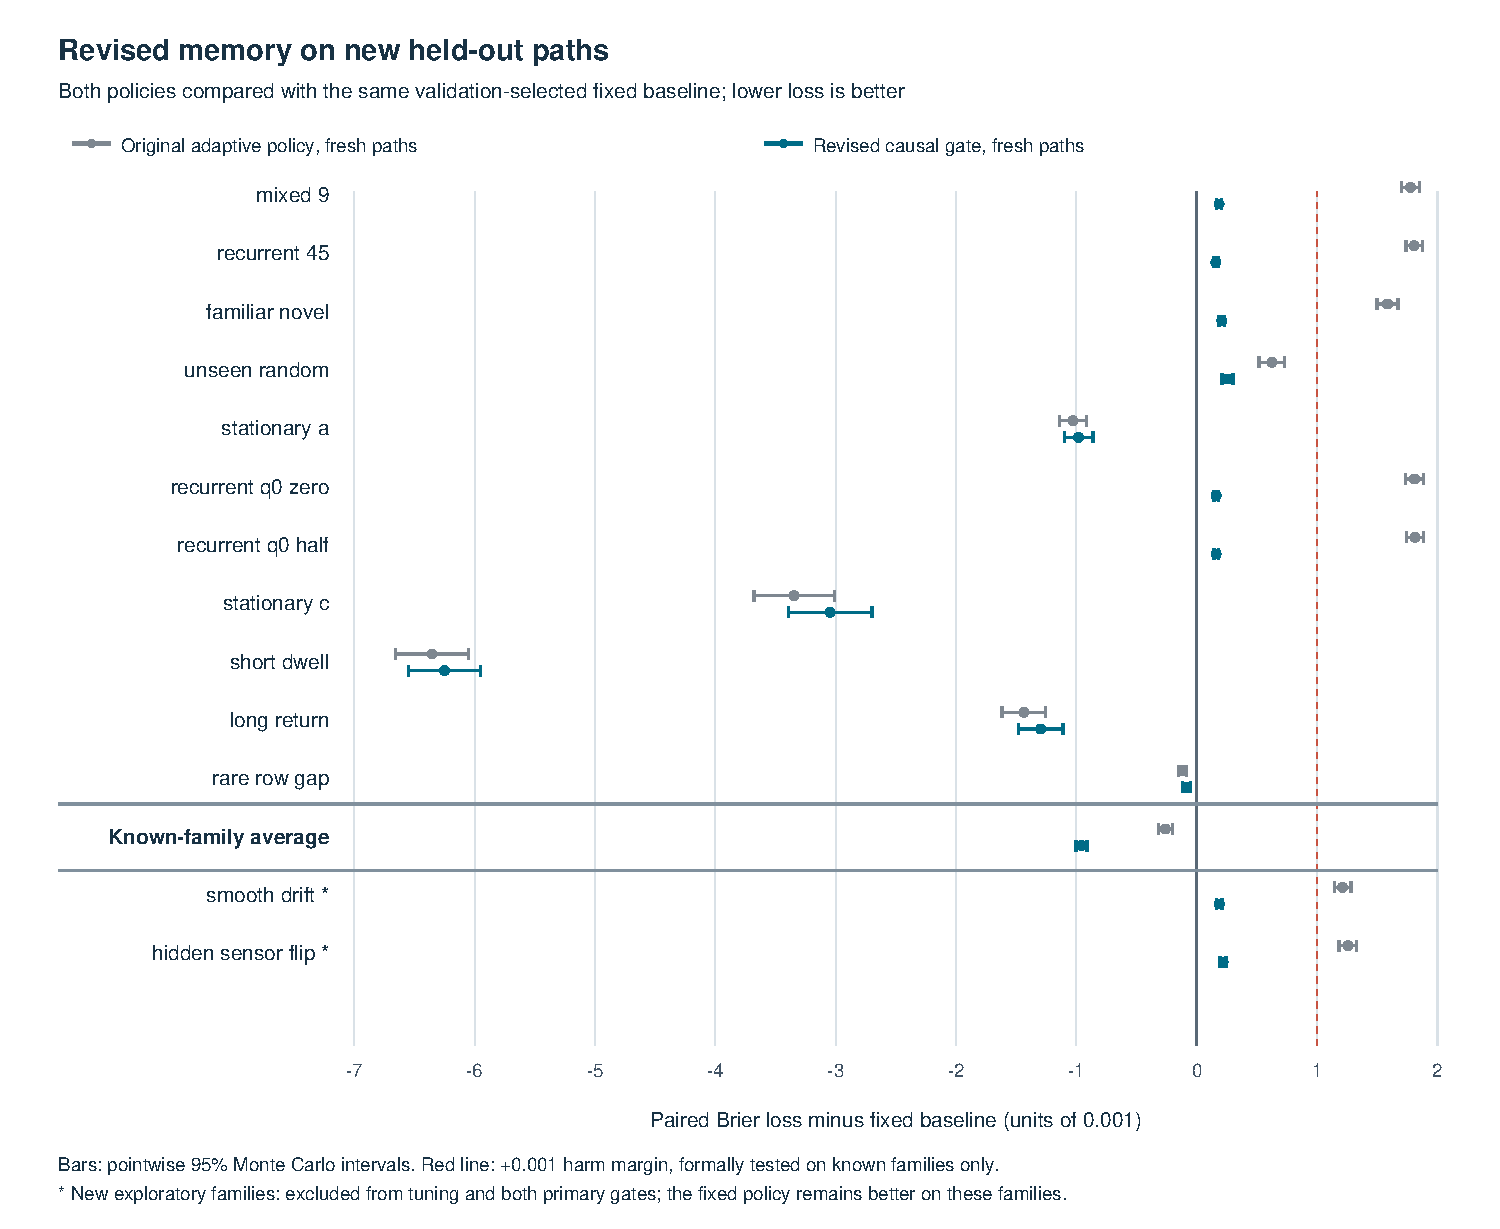
\includegraphics[width=\linewidth]{figures/revision_memory_results.pdf}
\caption{Matched fresh-path comparison of original and revised memory policies relative to fixed. The revised gate reduces large recurrent-family harms but modestly gives back some gains in other families. Bars are pointwise 95\% Monte Carlo intervals; formal gates use separately computed simultaneous bounds. The starred new transfer families were excluded from selection and both primary gates, and fixed remains better on them.}
\label{fig:revision-memory}
\end{figure}

There is no uniform domination. Six known-family mean differences remain positive relative to fixed, although their simultaneous bounds lie within the chosen harm margin. Revised minus original adaptive mean loss is positive in five known families: \texttt{stationary\_a}, \texttt{stationary\_c}, \texttt{short\_dwell}, \texttt{long\_return}, and \texttt{rare\_row\_gap}. The largest giveback is $+0.000299956$ in \texttt{stationary\_c}; \texttt{short\_dwell} worsens by $+0.000104135$. In these families the revised policy still has lower mean loss than fixed. In the two new transfer families, revised minus original adaptive is $-0.00102356$ and $-0.00103747$, but revised minus fixed is $+0.000187958$ and $+0.000218210$. These exploratory outcomes favor the revision over its adaptive predecessor while retaining a counterexample to superiority over fixed.

All fifty-one software checks passed: forty-one inherited checks and ten gate-specific tests, including current-outcome and future-suffix invariance, invalid-input nonmutation, convex-hull/normalization checks, and controls that detect update-before-predict and reversed-loss weighting. The audit reproduced validation selection, replayed 11,640 gate steps from twenty-six full traces, and checked seventy-eight trace-score/hash pairs. Independent aggregate arithmetic reproduced seed-cluster means, intervals, and the simultaneous harm calculation from the per-path losses. All 1,300 paths retain scores and forecast/stream hashes; the twenty-six traces contain full observations and forecasts.

The experiment took about 259 seconds, plus about six seconds for correctness checks. Held-out revised computation, including both experts and the gate, totaled 102.27 seconds versus 72.63 seconds for the original adaptive expert alone, approximately $1.41\times$. Gate-only overhead was 2.03 seconds and is not the cost of deploying the full revision. These machine timings include verification overhead and are descriptive. The result establishes a bounded improvement under the specified generator mixture and selection protocol, with remaining harms and transfer limits.


\subsection{Interpretation and remaining boundaries}
The revision experiments address engineering parts of Z1 and Z3, with different coverage. The two semantic tests directly compare old and revised single-pass systems, but their primary target is fewer erroneous definite judgments under three additional safeguards. Both candidates fail that joint target on their own fresh holdouts; the second removes the targeted false refutations of undecidable claims at the cost of unnecessary abstentions and persistent negation errors. Neither replaces Z1's original abstention-reduction endpoint, supplies a rules-by-schema factorial ablation, or provides independent human labels. Z2's claimed advantage from role diversity and Z4's metadata-ablation prediction remain unresolved. For Z3, the revised algorithm passes the original numerical criterion on new paths as well as its separate repair criterion. It does not establish superiority over all memory policies, every generator, or real agent memory workloads.

These outcomes must remain attached to the exact revisions, comparators, and test sets. The memory transfer failures motivate subsequent evaluation on externally sourced temporal tasks, with validation and final test partitions fixed before tuning. The semantic comparisons call for independently adjudicated cases, richer source packets, adversarial scope changes, negated-claim controls, guard-specific ablations, and resource-matched comparisons. Neither favorable local result nor an internal freeze supplies general deployment assurance. All current cases and simulation families are now exposed evaluation material and must not be reused as a fresh confirmatory holdout for a later tuned revision.

All revisions are additive local research implementations. No installed model weights, external services, synced project sources, or production workflow were changed. The paper reports behavior under the saved code and test protocols; the new archive supplies the exact revision for inspection and reproduction. The earlier physical-model calculations are preserved but not rerun in this revision campaign. Improvements in evidence judgments or synthetic prediction loss would not supply a scalar-field observation, machine-consciousness measurement, or physical validation of a Theory of Everything.
